\section{Model Generalization for Other Polar Surfaces}

According to Figure \ref{Chap:ZnO_H:fig:doped}, in a (2$\times$2) supercell of ZnO (000$\overline{1}$) surface, if one Zn atom is replaced by one metallic dopant atom with 1 (Na), 2 (Mg), 3 (Al) and 4 (Ti) valence electrons, the critical $\theta_{\textup{H}}$ for the metal-semiconductor transition and the abrupt change of $E_{\textup{ad}}^{\textup{H}}$, denoted as  $\theta_{\textup{H}}^{\textup{c}}$, is $\frac{3}{4}$,  $\frac{1}{2}$, $\frac{1}{4}$ and 0 ML, respectively. $\theta_{\textup{H}}^{\textup{c}}$ is simply obtained by the requirement that all O atoms on the top surface layer should be fully saturated in closed-shell electron configuration according to the electron counting model. Thus, $\theta_{\textup{H}}^{\textup{c}}$ can be calculated for other (000$\overline{1}$) surfaces of wurtzite structures, ($\overline{1}$$\overline{1}$$\overline{1}$) surfaces of zincblende structures, and other semiconductor surfaces with two separate sublattices (one for cations and one for anions) and only the anions (O, N, S, etc.) on the top surface layer (\emph{polar semiconductor surfaces}). Generally, with $n_{\textup{dopant}}$ types of dopant elements in bulk lattice, $\theta_{\textup{H}}^{\textup{c}}$ can be calculated in the unit of ML as the following
\begin{equation}
  \begin{array}{rcl}
      \theta_{\textup{H}}^{\textup{c}}&=&(\frac{8}{N_{\textup{bond}}}-\frac{1}{N_{\textup{bond}}}V_{\textup{anion}})\times1.0\textup{ML}\\\\
      &&-\sum_{i=1}^{n_{\textup{dopant}}}\theta_{\textup{dopant}}^i(V_{\textup{dopant}}^i-V_{\textup{cation}})\\
  \end{array}
  \label{eq3}
\end{equation}
Here $V_{\textup{cation}}$, $V_{\textup{anion}}$ and $V_{\textup{dopant}}^i$ is the number of valence electrons for the cation element in bulk lattice, the anion element in bulk lattice and the dopant cation element $i$, respectively. $N_{\textup{bond}}$ is the number of bonds between one cation (anion) and its nearest anion (cation) neighbors in bulk lattice. $\theta_{\textup{dopant}}^i$ is the concentration of the dopant element $i$ per surface area (in unit of ML). For a Al-doped ZnO (000$\overline{1}$) surface that has only one Al atom in a (2$\times$2) supercell, $N_{\textup{bond}}$ = 4, $V_{\textup{cation}}$ = 2, $V_{\textup{anion}}$ = 6, $n_{\textup{dopant}}$ = 1, $V_{\textup{dopant}}^1$ = 3 and $\theta_{\textup{dopant}}^1$ = $\frac{1}{4}$ ML, so $\theta_{\textup{H}}^{\textup{c}}$ = $\frac{1}{4}$ ML according to Equation \ref{eq3}, consistent with Al-doped result in Figure \ref{Chap:ZnO_H:fig:dop1}. 

Equation \ref{eq3} can be easily extended to the cases with multiple dopant elements ($n_{\textup{dopant}} > 1$). For example, if two Zn atoms at bulk Zn substitutional sites are replaced by one Al dopant atom and one Ti dopant atom in a (2$\times$3) supercell of ZnO (000$\overline{1}$) surface, $n_{\textup{dopant}}$ = 2,  $V_{\textup{dopant}}^1$ = 3, $V_{\textup{dopant}}^2$ = 4, and $\theta_{\textup{dopant}}^1$ = $\theta_{\textup{dopant}}^2$ = $\frac{1}{6}$ ML,  so $\theta_{\textup{H}}^{\textup{c}}$ = 0 ML according to Equation \ref{eq3}. This prediction is confirmed by our calculations of H adsorption strength on this Al-Ti-doped ZnO (000$\overline{1}$) surface shown in Figure \ref{Chap:ZnO_H:fig:2dop}. 

Equation \ref{eq3} can also be easily extended to the cases of other defects such as vacancies. For example, recently it was reported that a stable ZnO (000$\overline{1}$) surface configuration has $\frac{1}{3}$ ML Zn vacancies and 10 H atoms in a (3$\times$3) (000$\overline{1}$) surface unit cell \cite{Jacobs16ZnO}. Here the Zn vacancy can be regarded as a type of dopant cation with zero valence electron. Using the corresponding parameters ($N_{\textup{bond}}$ = 4,$V_{\textup{anion}}$ = 6, $n_{\textup{dopant}}$ = 1, $\theta_{\textup{dopant}}$ = $\frac{1}{3}$ ML, $V_{\textup{dopant}}$ = 0 and $V_{\textup{cation}}$ = 2), $\theta_{\textup{H}}^{\textup{c}}$ = $\frac{7}{6}$ ML according to Equation \ref{eq3}, corresponding to 10.5 H atoms in a (3$\times$3) ZnO (000$\overline{1}$) surface unit cell. It means the adsorption of the 11th H atom in this unit cell would be too weak to occur under normal environment conditions, consistent with the experimental observations and \ac{DFT} calculations \cite{Jacobs16ZnO}.

\begingroup
\begin{figure}[!ht]
  \centering
  \subfigure[]{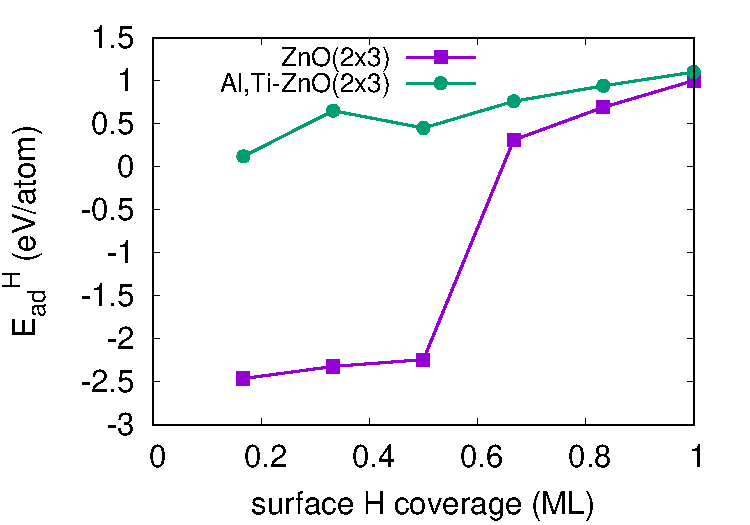
\includegraphics[width=0.7\linewidth]{Chap1/plots/Eadh_2x3_H.pdf}}\label{Chap:ZnO_H:fig:2dop}
  \subfigure[]{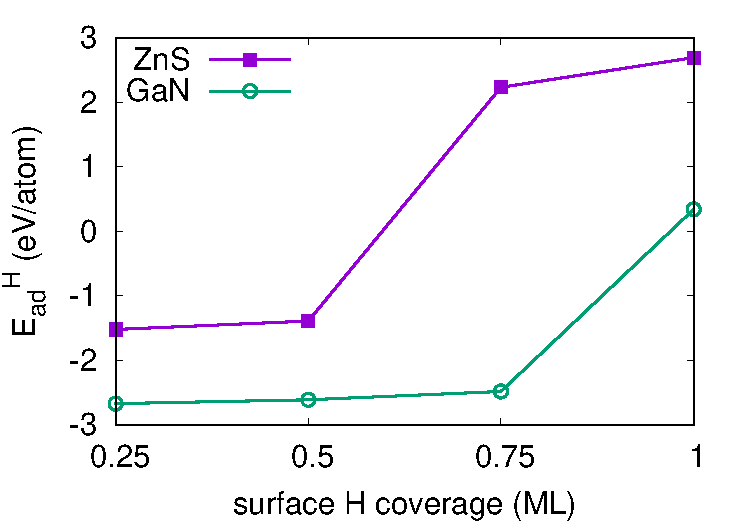
\includegraphics[width=0.65\linewidth]{Chap1/plots/E_C_4.pdf}}\label{Chap:ZnO_H:fig:otherads}
\caption[$E_{\textup{ad}}^{\textup{H}}$ on (2$\times$3) ZnO (000$\overline{1}$) surface with the co-existence of 1 Al substitutional dopant atom and 1 Ti substitutional dopant atom at bulk Zn sites.]{$E_{\textup{ad}}^{\textup{H}}$ on (2$\times$3) ZnO (000$\overline{1}$) surface with the co-existence of 1 Al substitutional dopant atom and 1 Ti substitutional dopant atom at bulk Zn sites. (a):$E_{\textup{ad}}^{\textup{H}}$ on (2$\times$2) zincblende ZnS ($\overline{1}$$\overline{1}$$\overline{1}$) and wurtzite GaN (000$\overline{1}$) surfaces with different $\theta_{\textup{H}}$. }
  \label{Chap:ZnO_H:fig:others}
\end{figure}
\endgroup

The electron counting model and Equation \ref{eq3} can be used to explain the H adsorption strength on other polar semiconductor surfaces. For example, sulfur(S)-terminated ($\overline{1}$$\overline{1}$$\overline{1}$) surface of zincblende ZnS have the similar atomistic structure and valence electron configuration as those for wurtzite ZnO (000$\overline{1}$). As shown in Figure \ref{Chap:ZnO_H:fig:otherads}, the dramatic decrease of H adsorption strength happens when $\theta_{\textup{H}}$ increases from $\frac{1}{2}$ to $\frac{3}{4}$ ML, the same as ZnO in Figure \ref{Chap:ZnO_H:fig:Ead}. Moreover, for nitrogen(N)-terminated (000$\overline{1}$) surface of wurtzite GaN, because each N atom has 5 valence electrons and 4 Ga-N bonds, $\frac{8-5}{4}$ = 0.75 electron is required to saturate each N atom on (000$\overline{1}$) surface once the GaN bulk lattice is chopped into two surfaces along [0001] direction. According to Equation \ref{eq3}, $N_{\textup{bond}}$ = 4, $V_{\textup{anion}}$ = 5, and $\theta_{\textup{dopant}}^i$ = 0 ML, so $\theta_{\textup{H}}^{\textup{c}}$ = $\frac{3}{4}$ ML . Therefore, $\theta_{\textup{H}}$ = $\frac{3}{4}$ ML, equivalent to 3 hydrogen atoms in the supercell of a (2$\times$2) GaN (000$\overline{1}$) surface, can transform all 4 surface N atoms from metallic to semiconductor states. Correspondingly, the hydrogen adsorption strength decreases dramatically when $\theta_{\textup{H}}$ increases from $\frac{3}{4}$ to 1 ML as shown in Figure \ref{Chap:ZnO_H:fig:otherads}. 